\documentclass[ngerman,aspectratio=169,10pt]{beamer}

\usetheme[progressbar=frametitle]{metropolis}
\usepackage{appendixnumberbeamer}

\graphicspath{{./graphics/}, {./../../figures/}}

\usepackage{booktabs}
\usepackage{xspace}
\usepackage{amsmath}
\usepackage{amssymb}
\usepackage{amsthm}
\usepackage{xfrac}
\usepackage{listings}
\lstset{
	basicstyle=\ttfamily,
	showstringspaces=false,
	tabsize=4,
	upquote=true,
}

\title{ILP-Solver für das Labeling-Problem}
% \subtitle{}
\date{13. Januar 2021}
\author{Levin Nemesch, Joshua Sangmeister}
\institute{Algorithm Engineering - Projekt}
\titlegraphic{
    \hfill
\includegraphics[height=1.5cm]{unilogo.pdf}\\
    \hspace*{8.3cm} \textsc{AG Theoretische Informatik}
}

\begin{document}

\maketitle

\begin{frame}{ILP-Formulierung}
	\textbf{Variablen}:
    \begin{itemize}
        \item $P$: Menge aller Punkte
        \item $C$: Menge aller Kandidaten
        \item $C_p$: Alle Kandidaten des Punktes $p$
    \end{itemize}

	\begin{align*}
	\max && \sum_{c\in C}x_c&&\\
	\text{s.t.} && \sum_{c\in C_p}x_c &\leq 1 &\forall p\in P\\
	&& x_{c_1} + x_{c_2} &\leq 1 &\forall c_1, c_2\in C \mid \text{$c_1$ and $c_2$ overlap}\\
	&& x_c &\in\{0,1\} &\forall c\in C
	\end{align*}
\end{frame}

\begin{frame}[fragile]{Callback-Heuristik}
    Relaxierte Lösung des ILP gegeben, dazu treshold $t$:
    \begin{verbatim}
    for each point in order:
        sort Cp descending
        for c in Cp:
            if c > t and no conflict with any predecessor:
                c = 1
                set all in Cp\{c} = 0
                break
    \end{verbatim}
    \onslide<2>{
    Treshold $t$?
    \begin{itemize}
        \item Hoch: Punkt kann auch gar nicht gelabelt werden, wenn $C_p$ sehr "unentschlossen"
        \item Niedrig: Punkt wird nach Möglichkeit gelabelt, $C_p$ wird als Ranking nach Erfolgswk. gedeutet
    \end{itemize}
    }
\end{frame}

\begin{frame}{Güte der SA-Heuristik}
    \centering
    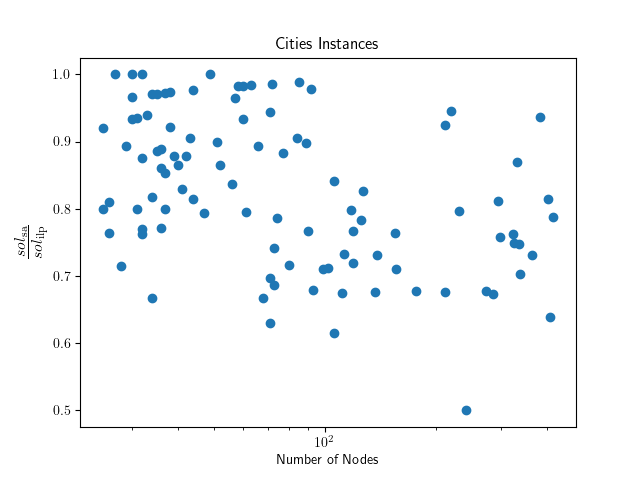
\includegraphics[width=270px]{value_sa_vs_ilp}
\end{frame}

\begin{frame}{Laufzeit ILP vs. SA}
    \centering
    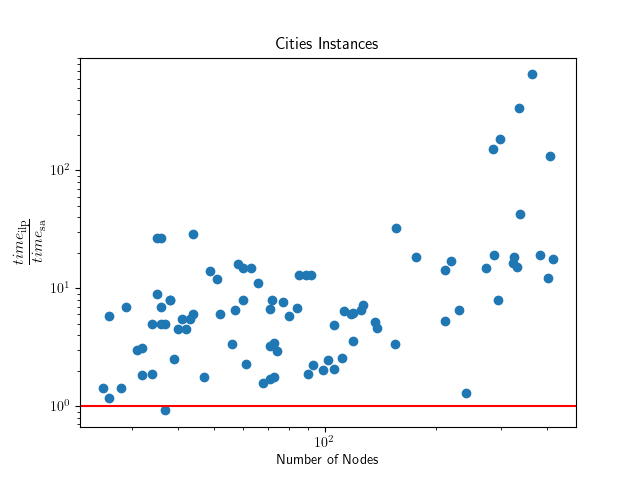
\includegraphics[width=270px]{time_ilp_vs_sa}
\end{frame}

\begin{frame}{Laufzeit mit/ohne Callback-Heuristik}
    \centering
    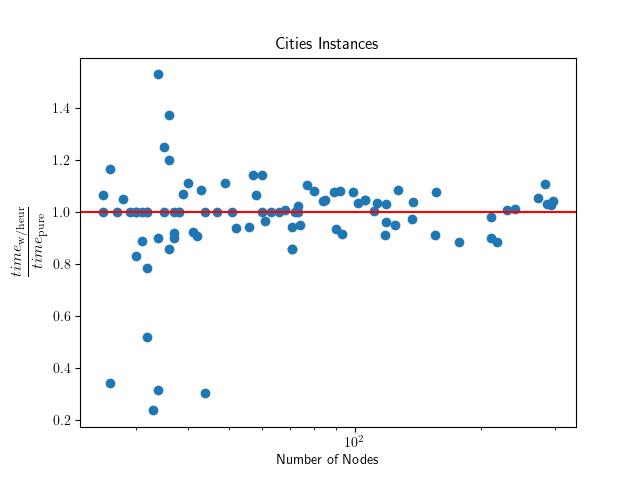
\includegraphics[width=270px]{time_heuristic_vs_pure}
\end{frame}

\begin{frame}{Laufzeit verschiedener Parameter}
    \centering
    \begin{columns}
        \begin{column}{0.6\linewidth}
            \vspace{10px}
            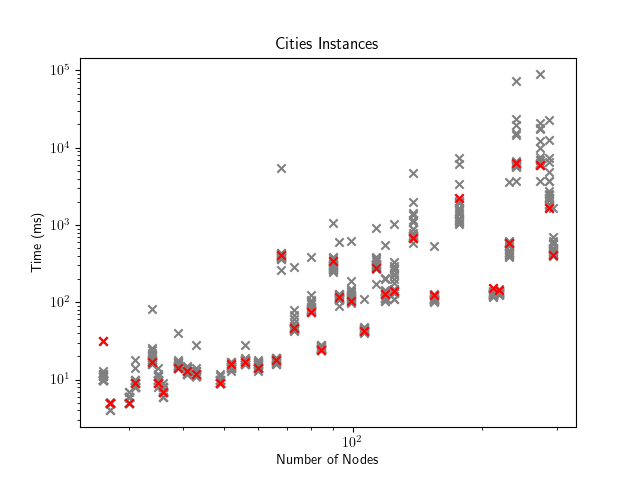
\includegraphics[width=270px]{time_ilp_parameters}
        \end{column}
        \begin{column}{0.2\linewidth}
            Parameter:
            \begin{itemize}
                \item Concurrent
                \item Focus
                \item Method
                \item Cuts
                \item Presolve
            \end{itemize}
        \end{column}
    \end{columns}
\end{frame}

\begin{frame}{ILP als Heuristik}
    Setze timeout, übernehme dann bisherige beste Lösung des Solvers:
    \begin{itemize}
        \item Für einige mittelgroße Instanzen bessere Lösungen als SA-Heuristic
        \item Große Instanze weiterhin problematisch
        \item Black-Box-Magie, unklare Gütegarantien
    \end{itemize}
\end{frame}

\begin{frame}{Ausblick - Verstärkende Ungleichungen}
    \begin{figure}
        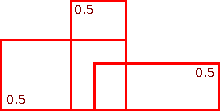
\includegraphics[width=180px]{verstaerkend1}
    \end{figure}
    Relaxierte (Teil-)Lösung ist gültig
\end{frame}

\begin{frame}{Ausblick - Verstärkende Ungleichungen}
    \begin{figure}
        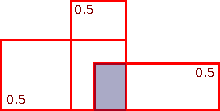
\includegraphics[width=180px]{verstaerkend2}
    \end{figure}
    Neue Ungleichung für Punkt auf blauer Fläche, beschränke dort Summe aller Label auf 1
\end{frame}

\begin{frame}{Ausblick - Verstärkende Ungleichungen}
    \begin{figure}
        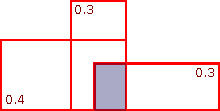
\includegraphics[width=180px]{verstaerkend3}
    \end{figure}
    Rettet uns aber nicht vor anderen Relaxierungen
\end{frame}

\end{document}